\documentclass[english, kiv, sem, he, iso690alph, pdf, viewonly]{fasthesis}
\title{Lisp language subset interpret}
\author{Jan}{Hejdušek}
\supervisor{Ing. Kamil Ekštein, Ph.D.}
\assignment{sw2025-02.pdf}

\usepackage{csquotes}
\usepackage{pdfpages}

\nobastardtitle
\nocopyrightnotice

\newif\iffullbuild
\fullbuildtrue

\lstset{style=FASThesisLstStyle, numberblanklines=false, tabsize=5,
keywordstyle=\color{red}}

\begin{document}
\iffullbuild
\frontpages[notm]
\tableofcontents
\fi

\chapter{Introduction}
\section{Overview}
This paper is a documentation for a seminar work in course KIV\slash
PC -- Programming in C language. I will cover the assignment itself,
analysis of the problem, details of the implementation, short guide
for building and running the application and finally a conclusion
covering how the work went.
\section{Assignment}

The assignment for this seminar work is to develop a console
application in the C~programming language that interprets a subset of
the Lisp programming language (hereafter referred to only as Lisp).
The complete assignment, in Czech, is provided at the end of this document.

\chapter{Analysis}
\section{Statement}
As stated, the primary objective is to design and implement an
interpreter for a~subset of Lisp. The interpreter must be capable of
processing source code provided
either in a file or interactively via a command--line interface.

We will need to correctly parse the source code, thus analyze the
Lisp grammar and use an appropriate parser for it.
Design a data structure to represent the parsed source code and
correctly evaluate it.

\section{Lisp Grammar}
Our Lisp strictly follows a fully parenthesized prefix notation
(except for a quote) and Expressions in our Lisp can only be either a
constant, list or a
symbol\slash~string identifier, for example:
\lstinline|(1 is a constant and (this is a list of symbols))|.
If we treat operators the same way as variable identificators
we can describe the structure vith a simple context free grammar(CFG).
\label{fig:grammar}
\begin{align*}
  L & \rightarrow EL \mid \epsilon                    \\
  E & \rightarrow\ \texttt{'}E \mid (L) \mid C \mid S \\
  C & \rightarrow \textit{constant}                   \\
  S & \rightarrow \textit{string identifier}
\end{align*}
However by those rules we can also create expressions that are not
part of our Lisp.  Meaning if we parse the source code acording to
this grammar, we will
miss on some syntax errors that will be necessary to catch during evaluation.

We could also design much more complex grammar that could also categhorize
the oparators and function calls, check correct number of arguments and more.
With this we coul find additional syntax errors in the source code,
for example that conditions expexting T or NIL
\footnote{T and NIL are special values use by Lisp to indicate
true\slash~false or an empty list}.
However most of those syntax errors could still happen in runtime due
to nature of variables in Lisp.
Because variables can be passed almost everywhere and can contain any
valid Lisp expression.
Meaning we will have to check for those syntax errors during runtime anyway.

For our purpose, the simple grammar is sufficient enough. With the
tradeof of how easy to parse it is. For the parsing itself, we can
use any known parser for parser for CFG grammars. We prefer a
top--down parser, as we build the tree from root.

Since lookahead is not required (where an LL(1)\slash LL(k) parser
would be useful), parsing is possible without backtracking; the
parser can abort when an unbalanced parenthesis is detected,
therefore a recursive descent parser can be used.

Complex grammar and other parsers could be better if we would like to
expand the grammar, but in this scale, we chose the simplicity.

\section{Syntax Tree}
We will need to design a data structure capable of representing the
Lisp expressions
that will later be possible to traverse and evaluate. For such
structure there are multiple options:
\begin{enumerate}
  \item \textbf{Binary tree\slash s--expression}: One child
    represents a value of the node
    or contain another node and the other child would work as a
    linked list. See \ref{fig:ast_example2}
  \item \textbf{N--ary tree}: Each node can have an arbitrary number
    of children,
    matching the parenthesis structure. Each list is a node with
    children for each item of the list. See \ref{fig:ast_example}
  \item \textbf{Stack based}: The operands and operators
    could be together
    with parenthesis pushed into a stack and retrieved for each operator.
\end{enumerate}

We will not discuss Stack based evaluation further as it would be
hard to manage loops,
unevaluated parts of the code and quite an overhead would be
necessary to keep track of current operations.
Essentially we would be building our own call stack and the solution
would not be better than other options.

\begin{figure}[h]
  \centering
  \begin{minipage}{0.48\textwidth}
    \centering
    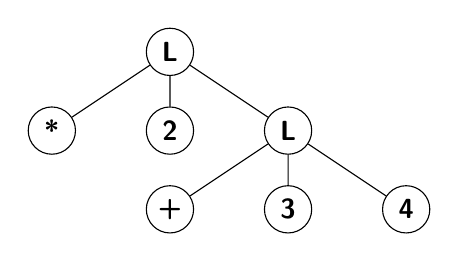
\begin{tikzpicture}[
        every node/.style={draw, circle,minimum size=0.6cm, inner
        sep=0pt,font=\sffamily\bfseries},
      level distance=1cm, ]
      \node {L}
      child { node {*} }
      child { node {2} }
      child { node {L}
        child { node {+} }
        child { node {3} }
        child { node {4} }
      };
    \end{tikzpicture}
    \caption{N--arry syntax tree representing \texttt{(* 2 (+ 3 4))}}
    \label{fig:ast_example}
  \end{minipage}
  \hfill
  \begin{minipage}{0.48\textwidth}
    \centering
    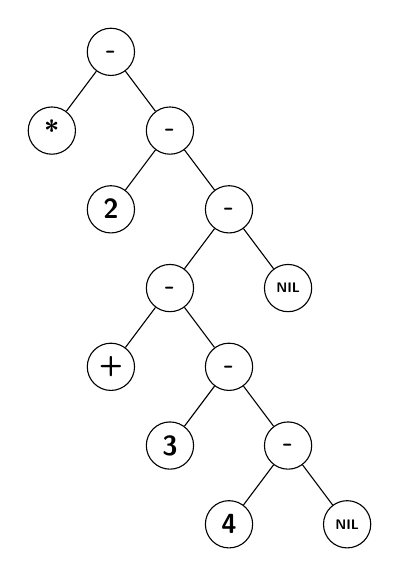
\begin{tikzpicture}[
        every node/.style={draw, circle, minimum size=0.6cm, inner
        sep=0pt, font=\sffamily\bfseries},
      level distance=1cm, ]
      \node {-}
      child { node {*} }
      child { node {-}
        child { node {2} }
        child { node {-}
          child { node {-}
            child { node {+} }
            child { node {-}
              child { node {3} }
              child { node {-}
                child { node {4} }
                child { node {\tiny{NIL}} }
              }
            }
          }
          child { node {\tiny{NIL}} }
        }
      };
    \end{tikzpicture}
    \caption{S--expression syntax tree representing\texttt{(* 2 (+ 3 4))}}
    \label{fig:ast_example2}
  \end{minipage}
\end{figure}

\subsection{S--expression}
Lisp is originally designed with s(symbolic)--expressions in mind as
its internal structure and many of its functionalities are based on it.
Syntax tree represented as an~S--expression has few specific features.

Some traversals of the syntax tree are dificult to make, for example
right to left traversal requires either back--links or accumulating children.
Since every list is essentailly a~linked list, access time to its
items is $O(n)$ where $n$ is index if the item,
also we do not know the size of the list without going through all the nodes.

The 'NIL' object used in Lisp also appears naturally in the
s--expression as a list terminator.
Also for example the function \lstinline|CDR| returning a list without
the first item is straightforward to implement as it is just the 'tail' node.

\subsection{N--ary Tree}
N--ary tree is a natural way to represent a nested parenthesized
lists structure and quite universal.
Having all list items in one array is pleasant to work with and it
is straightforward to traverse an abstract syntax tree(AST) in any order.
It ouperforms s--expresson in both time and memory for large lists,
$O(1)$ access time to list items and not using as many nodes.

However for this our purpose, it is not practikal exactly where
s--expression and Lisp behave specifically.
Dynamically allocating arrays and coppying data for the lists is more compplex
than in s--expression where it may be just changing one reference to a node.

\label{sec:nary-crd}
The \lstinline|CDR| function requires either having a counter at each node
if it was cdr'd during evaluation and checking it on every other operation
or to create a dummy list node and copy all the remaining references in a list.
With the \lstinline|CDR| function it gets even more complex when we
want to use it for changing content of variables
where we want to replace a whole part of a list with something
else(which is again straightforward in s--expressions).

For the implementation, we will use the n--ary tree, mainly because
it is more intuitive to work with and clear to traverse.
Getting a list item in \lstinline|O(1)| rather that
\lstinline|O(n)| is great, but not essential for our purpose.
These advantages overweight the s--expression, and the few specific
behaviors of Lisp should not be dificult to implement.

\section{Evaluation}
Lisp expressions can evaluate basically to any other Lisp expression.
We may expect the what the result of an evaluation is in some cases,
for example in expresstion \lstinline|(+ x y)| x and y should be
numbers, but mostly we do not have information what will the result be.
Based on this the result of an expression needs to be a generic expression.
So we will need an unified evaluation function.

With a better classification of symbols and function operators,
either by grammar, parsing or at runtime. We could split the
evaluation functions based on their return type. However that is not
necessary for the purposes of simple Lisp interpreter.

\chapter{Implementation}
\section{Architecture Overview}
The interpreter is divided into several modules:
\begin{itemize}
  \item \textbf{Preprocessor}: Removes comments and normalizes input.
  \item \textbf{Lexer}: Tokenizes source code into tokens.
  \item \textbf{Parser}: Converts token array into an AST according
    to the grammar.
  \item \textbf{AST Module}: Utils for creating, copying, and freeing AST nodes.
  \item \textbf{Environment}: Manages variable storage and lookup.
  \item \textbf{Operators}: Implements Lisp functions and
    arithmetic/logical operators.
  \item \textbf{REPL}: Read--eval--print loop.
\end{itemize}
See \ref{fig:workflow} for workflow diagram of the program.

\subsection{Used Data Dtructures}
\subsubsection{AST Node}
The AST node represents a general Lisp expression. Its structure is as follows:
\begin{itemize}
  \item \textbf{Type field (\lstinline|node.type|):} Specifies what
    the node represents and what is stored inside the union field.
  \item \textbf{Union field (\lstinline|node.as|):} Node data,
    depending on the node type:
    \begin{itemize}
      \item \lstinline|value| (\lstinline|int|): Used for numbers and booleans.
      \item \lstinline|symbol| (\lstinline|char*|): Used for symbol nodes.
      \item \lstinline|list|: Contains two fields:
        \begin{itemize}
          \item \lstinline|children| (\lstinline|struct ASTnode **|):
            Array of pointers to child nodes.
          \item \lstinline|count| (\lstinline|int|): Number of
            children in the list.
        \end{itemize}
    \end{itemize}
  \item \textbf{Origin field (\lstinline|node.origin|):} Used for
    memory management, marking whether the node is:
    \begin{itemize}
      \item Part of the original AST,
      \item A variable,
      \item A temporary evaluation result,
    \end{itemize}
\end{itemize}
For example, the first child of a list node can be accessed with \\
\lstinline|node.as.list.children[0]|.
See \ref{src:astnode} for struct definition in C language.

\begin{figure}[h!]
  \centering
  \includegraphics[width=.8\textwidth]{img/dataflow.pdf}
  \caption{Interpreter workflow}
  \label{fig:workflow}
\end{figure}

\begin{code}{C}{AST node struct\label{src:astnode}}
typedef struct ASTnode {
  enum node_type {
    BOOLEAN,
    NUMBER,
    SYMBOL,
    LIST,
  } type;
  enum node_origin {
    UNSET,
    AST,
    VARIABLE,
    TEMPORARY,
  } origin;
  union {
    int value;
    char *symbol;
    struct {
      struct ASTnode **children;
      int count;
    } list;
  } as;
} astnode;
\end{code}

\subsubsection{Operators}
\label{sec:operators}
Looking up the correct C functions for each Lisp operator(by operators
  also refering
to Lisp functions) is done using a \lstinline|struct operator_entry|
which maps a string to a~function. We keep an entry for each operator
in an array named \lstinline|operators|.

\subsubsection{Environment Variables}
Variables are stored as pairs of string(name of the variable) and
\lstinline|ASTnode| struct inside an array contained in
\lstinline|Env| together with count of existing variables. See
\ref{src:env} for C~source code.

\begin{code}{C}{Environment struct\label{src:env}}
struct var_record {
  char *symbol;
  astnode *node;
};

typedef struct Env {
  struct var_record *vars;
  int var_count;
} env;
\end{code}

\section{Macros and Error Handling}

An \lstinline|err_t| enum is used to several types of errors also
including the program exit status.
Throughout the entire source code macros are videly used for error
handling and returning \lstinline|enum err_t| from functions. See
\ref{src:errt} for possible values of \lstinline|err_t| enum.
See \ref{src:macros} for demonstration of how the macros are used.
The are currently 5 macros in use:
\begin{enumerate}
  \item \lstinline|RETURN_ERR_IF(cond, err)|
  \item \lstinline|RETURN_VAL_IF(cond, retval)|
  \item \lstinline|RETURN_NULL_IF(cond)|
  \item \lstinline|CLEANUP_WITH_ERR_IF(cond, label, err)|
  \item \lstinline|LOG_IF_VERBOSE(err)|
\end{enumerate}

The first 3 macros simply return given value, respectively NULL or an
error if the condition passes. \lstinline|CLEANUP_WITH_ERR_IF| macro
additionally jumps to label and sets variable retval to given err
instead of returning it. \lstinline|LOG_IF_VERBOSE(err)| macro is
used inside the macros, further described in \ref{sec:errorlog}

% tex-fmt: off
\begin{code}{C}{\lstinline|err_t| used error codes\label{src:errt}}
typedef enum {
  ERR_NO_ERROR = 0,          // successful completion, no error
  ERR_INVALID_INPUT_FILE,    // invalid or missing input file name/format
  ERR_SYNTAX_ERROR,          // error in Lisp source code
  ERR_FILE_ACCESS_FAILURE,   // cannot read/write to file
  ERR_OUT_OF_MEMORY,         // malloc/calloc/realloc failed
  ERR_INVALID_ARGS,          // invalid program CLI arguments
  ERR_INTERNAL,              // unexpected internal error (should not happen)
  ERR_RUNTIME_UNKNOWN_VAR,   // access to undefined variable
  ERR_NOT_A_VARIABLE,        // assignment target is not a variable node
  ERR_ZERO_DIVISON,          // division by zero in arithmetic operator
  ERR_UNKNOWN_OPERATOR,      // unsupported or unknown Lisp operator
  CONTROL_BREAK,             // control signal for (brk) inside loops
  CONTROL_QUIT,              // control signal for (quit) to exit program
} err_t;
\end{code}
% tex-fmt: on

\newpage
% tex-fmt: off
\begin{code}{C}{Common function structure returning \lstinline|err_t|\label{src:macros}}
err_t func(args) {
  /* sanity check */
  RETURN_ERR_IF(sanity_condition, ERR_INTERNAL);

  err_t err, retval = ERR_NO_ERROR;

  /* code that possibly allocs */

  CLEANUP_WITH_ERR_IF(early_return_condition, cleanup, ERR_NO_ERR);

  err = func_that_can_fail();
  CLEANUP_WITH_ERR_IF(err, fail_cleanup, err);

cleanup:
  free(stuff_to_free_on_success);
  return retval
fail_cleanup:
  free(sutff_to_free_on_falilure);
  return retval
}
\end{code}
% tex-fmt: on

\subsection{Error logging}
\label{sec:errorlog}
The added value of macros over putting the code into
\lstinline|if(cond){/* code */}|
, except the increased readability, is the ability to log
file name and line number when errors occur. Meaning that if we keep this
structure throughout the code, we can print the entire call stack
when an error is caught, which is very helpfull for the programmer.

This logging is done by the last used macro
\lstinline|LOG_IF_VERBOSE(err)| that prints the error message to
\lstinline|stderr| stream and any subsequent calls append to this
print. If we do not want to generate all the code for logging the
errors, we can turn it off via a~compile--time switch, which greatly
reduces the size of the final executable.

\section{Handling Input}
The interpreter supports two modes of input: reading from a file or
interactively from the command line. The mode is determined by
the command-line arguments provided at startup.

\subsection{Arguments}
The first argument of the file is alwais interpreted as a filename, it reads
the entire contents of the file into a buffer.
Optionally, a \lstinline|-v| flag can be provided as a second argument
to enable verbose output, printing the result of each evaluated
expression.

The argument parsing logic only checks for valid combinations
and prints usage help if the arguments are invalid. Finally the
buffer is passed to the evaluation pipeline for processing, which is
further handled by \lstinline|process_code_block| function.

\subsection{REPL}
If no argument is provided, the program enters an interactive
Read-Eval-Print Loop. In this mode, the interpreter repeatedly
prompts the user for input, reading lines from \lstinline|stdin|.
It accumulates lines until all parentheses are balanced, allowing for
multi-line expressions.

Once a complete expression is entered, it is
passed into \lstinline|process_code_block| function and essentially
treated in a same way as a source code from a file.
The REPL continues until either
evaluation of a \lstinline|(quit)| expression or an error occured
during evaluation and exits.

\section{Evaluation Pipeline}
Once a Lisp source code is obtained, we put it through a fixed
pipeline for parsing and evaluation. See \ref{fig:workflow}.
This pipeline is implemented in the \lstinline|process_code_block|
function and is
split into the following parts.

\subsection{Preprocessor}
The preprocessor is the first step in the pipeline. Its main purpose
is to normalize the input source code before tokenization and
parsing. It performs the following operations:
\begin{itemize}
  \item Strips Lisp comments starting
  \item Converts all alphabetic characters to uppercase
  \item Removes line separators
\end{itemize}
It does not shrink the size of the input string as it puts empty
spaces (character code 32).
These steps simplify subsequent tokenization and ensure consistent
behavior on Unix and Windows platforms.

\subsection{Lexer}
Lexer takes the normalized source code from preprocessor and
tokenizes it. The output is a null--terminated array of C strings
(\lstinline|char**| in C).

Splits on white spaces, tabs and creates standalone one--character
tokens from characters "\lstinline|'|", "\lstinline|(|" and "\lstinline|)|" .
It does not cathegorize the tokens.

\subsection{Parser}
For parsing we chose the grammar described above, see
\ref{fig:grammar}, and use recursive descent parser. The parser is
implemented vith two
functions \lstinline|parse_list| and \lstinline|parse_expr| for the
first two grammar rules and the rest is implemented in--place in the
\lstinline|parse_expr| function.
Those functions recursively call eachother and create AST nodes
corresponding to the parsed tokens and advance current token.

The parsing is initialized vith the \lstinline|parse_list| function
with all tokens. By starting with the rule $L \rightarrow EL \mid
\epsilon$ we also accept multiple expressions and an empty string.

\subsection{Evaluation}
The evaluation of a Lisp expression is unified for all node types. After
evaluating an expression, we once again obtain an expression.
Even the result of a simple sum of its arguments like
\lstinline|(+ 1 2 3)| % tex-fmt
is an AST node representing a Lisp expression.  Then we can
have an unified function for the evaluation:
\begin{code}{C}{Evaluation function\label{fun:eval}}
err_t eval_node(astnode *node, astnode **out_node, env *env)
\end{code}
The function takes an AST node as a parameter and returns another AST
node as an out--parameter.

When evaluating number and boolean nodes,
the node itself is returned as the out parameter.
When evaluating a symbol node, we treat it as a variable.
Using the \lstinline|env| struct, we get the variable content and
return it or exit with a syntax error when
the variable with this name does not exist in the environment.

For list nodes, we check the first child of the node if it is a
symbol and compare its value(string) with all known operators using the
\lstinline|operators| array described in \ref{sec:operators}.
If it matches an operator, we call its corresponding function, pass
the evaluated node to it and finally return the node we get from the
operator function. We return an error if no match is found.

\subsection{Operators}
All implemented functions handling Lisp operators share the same
signature(except function name) with evaluation function
\ref{fun:eval}. Their name has a prefix \lstinline|oper_| and then
keywords for the Lisp operators they implement, for example
\lstinline|oper_add|. It expects the
node parameter to be a list with the operator as first child. The
caller must free temporary parts of the result of evaluated nodes
when they can no longer be accessed, for details how the temporary
nodes are managed see \ref{sec:mem}.

Most of those functions evaluate the rest of child nodes in the list
and operate on the obtained values\slash nodes.
\paragraph{Arithmetic operators}
Operators \lstinline|+|, \lstinline|-|, \lstinline|*|, \lstinline|/|,
\lstinline|min| and \lstinline|max| get the values from
evaluated nodes (expected to be number nodes or an error is returned),
calculate the result and return a new number node.
Relational operators behave similarly, except that they return a boolean node.

Some operator functions are joined together and check the first
item of the list again to determine which operator it is. So that
there is not that much redundant code.

\paragraph{Function operators}
Functions \lstinline|quote|, \lstinline|atom|, \lstinline|car|,
\lstinline|nth| and \lstinline|length|
are straightforward. Except \lstinline|quote| they all evaluate the
second child,
\lstinline|atom| checks if it is not of type list, \lstinline|car|
returns its first child,
\lstinline|nth| returns its n--th child and \lstinline|length| returns field
\lstinline|node.as.list.child_count|.

The \lstinline|set| operator assigns a value to a variable in the
environment. The function first evaluates
the second child. If it is a symbol and does not exist in the
environment, it is initialized. If it is a node of
\lstinline|VARIABLE| origin, it is treated as the variable node to
replace. Then evaluates the value expression, and
makes a deep copy of the value node with origin \lstinline|VARIABLE|.
The previous content of the
variable is freed and replaced with the new value and
reference to the variable node is returned.

The \lstinline|cdr| and \lstinline|list| functions create a new
temporary list node and add
children to it. \lstinline|cdr| additionally frees the first skipped
node if its temporary.

\paragraph{Control functions}
Function \lstinline|if| evaluates 3rd or 4th child based on result of
2nd child, it expects to get a boolean node after evaluating the 2nd
child.

Function \lstinline|while| cyclically evaluates all children(except
the first one) in order, and stops
if the second one is \lstinline|NIL| or return value
\lstinline|err_t| of any evaluation is \\ \lstinline|CONTROL_BREAK|.

The \lstinline|brk| and \lstinline|quit| functions utilize the
already present error handling scheme and simply return a
\lstinline|CONTROL_BREAK| or \lstinline|CONTROL_QUIT|. Which is for
most operator functions just passed up as any normal error and those
error values are ignored by the macro logging logic.

\section{Memory Management}
\label{sec:mem}
For most modules and parts of evaluation, the memory management is
simple as we allocate and free in the same scope.
Tokenizing and parsing returns allocated data structures and it is up
to the caller to free them.

All structs we use have implemented their own free function, that
frees all parts which the struct contains and refers to.

During evaluation, where we need to create, allocate memory for new nodes
and return new evaluated Lisp expressions, we want to free the results
only sometimes. Respectively when the node is not a variable or part
of the original AST(we need to use it again when looping). For this
purpose the nodes are marked with an enum
\lstinline|node_origin|, see \ref{src:astnode} for the node struct definition.

Also temporary list nodes can contain subtrees that may or may not be
temporary. Then we need to free only its temporary parts. This
partial pruning is done using function \lstinline|free_temp_node_parts()|, which
frees the node if its temporary and recursively frees any its
temporary children. It does not search subtrees of non-temporary
nodes as those can not currently occur.

% We can not solve this by copying the result nodes during
% evaluation, because we need the
% original node when working with variables. For example
% \lstinline|(set (nth 1 arr) 1)| where \lstinline|arr| is a variable
% that contains a list node. We want to change only one of its
% children which would not work when we would make a copy during the
% \lstinline|nth| operation.

% \paragraph{ Problematic scenario }
% The expression \lstinline|(list 1 var (+ 1 2))| creates
% a temporary list node with one child from the original AST, one child
% is a variable from the
% environment and a one child is a temprorary result node.
% Using this expression for example in
% \lstinline|(nth 1 (list 1 var (+ 1 2)))| % tex-fmt
% we return the content of the variable. But the temporary
% result of \lstinline|(+ 1 2)| needs to be freed and \lstinline|nth|
% function does not access it.

% So every time we no longer use part of a node, we have to free all
% of its temporary subparts. For this there is a function
% \lstinline|free_temp_node_parts(node)|, which recursively frees
% everything in the node that has temporary origin;

\chapter{User guide}
\section{Compilation}

The source code follows the C99 standard and is designed to be
portable across platforms with a compliant C compiler. While the
application can be built using a standard toolchain, makefiles for
the GCC compiler are
provided for both GNU/Linux and Microsoft Windows environments.

\section{Execution}

The application supports two modes of operation: interactive mode and
batch processing.
Executing the program without arguments initiates the interactive
interpreter (REPL).
Alternatively, providing a file path as an argument processes the
contents of the specified file with Lisp source code.
A verbose execution mode, which prints results of outer expressions,
can be enabled by appending the \texttt{-v} flag when running with an
input file. Example of running the program in Linux environment on a
Lisp source code with bubble sort\footnote{The Lisp source code for
  the bubble sort algorithm was taken from the assignment at the end of
this document} algorithm:

\setuxprompt{hejdula@linux}{home}
\begin{console}{Example of running the program}
`\uxprompt` clisp.exe path/to/bubble_sort.lisp -v
[1]> (SET (QUOTE ARR) (QUOTE (2 5 1 9 0 8 3 7 4 6)))
(2 5 1 9 0 8 3 7 4 6)
[2]> (SET (QUOTE SWAPPED) T)
T
[3]> (SET (QUOTE LEN) (LENGTH ARR))
10
[4]> (WHILE SWAPPED (SET (QUOTE I) 1) (SET (QUOTE SWAPPED) NIL)
  (WHILE (< I LEN) (SET (QUOTE NUM1) (NTH (- I 1) ARR)) (SET (QUOTE
    NUM2) (NTH I ARR)) (IF (> NUM1 NUM2) (WHILE T (SET (NTH (- I 1)
ARR) NUM2) (SET (NTH I ARR) NUM1) (SET (QUOTE SWAPPED) T) (BRK))) (INC I 1)))
NIL
(0 1 2 3 4 5 6 7 8 9)
[5]> (PRINT ARR)
(0 1 2 3 4 5 6 7 8 9)
`\uxprompt`
\end{console}

\chapter{Conclusion}
\section{Functionality}
The work meets the objectives set by the assignment.
It delivers a functioning console interpreter for the specified subset of Lisp.
The implementation demonstrates appropriate memory management, error
handling and modularization.

\subsection{Test Runs}
The sample Lisp source code with bubble sort arlgorithm for small(10
items) array to sort, executes as expected under a milisecond.
For increasing number of items, runtime starts jumping up to seconds
at around a thousand. Maximum memory usage during the interpretation
stays allmost the same in both cases under 2MB. However the number of
all allocations with 1000 items was quite large around
7~milion, allocating 173MB in total.

\section{Expectations}
Throughout this whole work I expected to encounter many issues with
the C programming language, but to my surprise the opposite happened.
I am surprised how well it went with the programming itself, the
error handling with macros(that I am now glad I spent the time to
make them together with the logging)
was very usefull and saved me many and many hours that I would have spent
debugging the code.

In the end the work turned out much better than I expected it to be
given the limited time I had.

\section{Possible Improvements}
\paragraph{Reusing allocated memory for temporary results}
The dymanic allocating of memory for each temporary node is not
optimal. Assuming from the number of allocations in the test runs,
the allocating takes the most of the execution time by far.
The allocated memory could be reused when reevaluating the same
expression in original AST multiple times, which could greatly
increase the performance.

\paragraph{List joining with CDR function}
Later in the work I stumbled on a very specific thing that I had
no idea it should work in Lisp.
Joining lists in variables using \lstinline|cdr| function that is
mentioned in the analysis \ref{sec:nary-crd}.
I tried to implement it into the current implementation, but quite a
lot of stuff would need to be additionally handled
during the evaluation to properly add this feature and I gave up on
it.

\paragraph{Redundant code in operators module}
In the operators module, the unified structure for evaluation is
great, but it feels like there is a lot of redundant code.
Where manjority of those functions do the same with little variation.

I am not sure how the structure could be changed such that code in
those functions is less repetetive with the rest of the current structure.
One improvement would be possible if the parsing and grammar would be
more complex and would also distinguish the different function
operators during parsing. Then we could cathegorize those functions
to some with similar behavior and for example centralize evaluating
the arguments before passing it to the function.

That would be more scalable and overall better structured, but when
implementing it felt like an overkill for project of this scale that
I do not intend to further develop.

\section{Dificulties}
There are only a few things that were annoying during the work.
I did not anticipate well what scale would this project be and it
took longer than expected for a seminar work.
If this would be my first experience with C language, I would
probably end up refactoring
the codebase a few times. I also underestimated how much research and
analysis needed to be done before I started implementing.

Other than that no larger problems were encountered.

\label{assignment}
\includepdf[pages=-]{sw2025-02.pdf}
\end{document}
